
\section{Bow shocks from anisotropic wind--wind interactions}
\label{app:ancantoid}
\begin{figure}
  \centering
  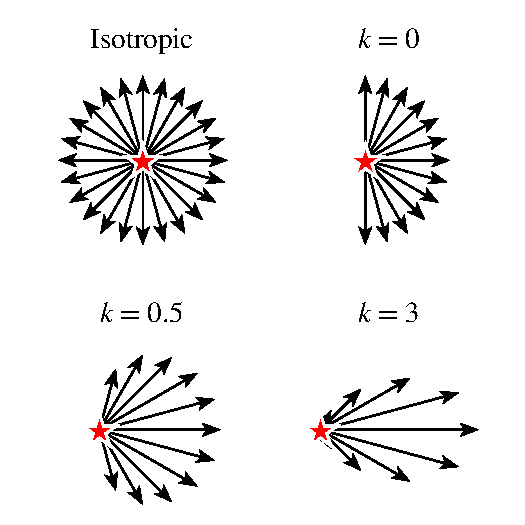
\includegraphics[width=\linewidth]{figs/anisotropic-arrows}
  \caption[]{Schematic diagram of wind flow patterns in isotropic and
    non-isotropic cases for different values of the anisotropy index,
    \(k\).  Arrow length represents the wind momentum loss rate per
    solid angle.}
  \label{fig:anisotropic-arrows}
\end{figure}


We wish to generalize the results of \citet[\CRW{}]{Canto:1996} to the
case where the inner wind is no longer isotropic, but instead has a
density that falls off with angle, \(\theta\), away from the symmetry axis.
Specifically, at some fiducial radius, \(r_0\), from the origin, the
wind mass density is given by
\begin{equation}
  \label{eq:ancantoid-density}
  \rho(r_0, \theta) =
  \begin{cases}
    \rho_0 \cos^k \theta & \text{for \(\theta \le 90^\circ\)} \\
    0 & \text{for \(\theta > 90^\circ\)}
  \end{cases}
  \ ,
\end{equation}
where \(\rho_0\) is the density on the symmetry axis and \(k \ge 0\) is an
\textit{anisotropy index}.  The wind velocity is still assumed to be
constant and the wind streamlines to be radial, so the radial
variation of density at each angle is
\(\rho(r, \theta) = \rho(r_0, \theta)\, (r/r_0)^{-2}\) and the wind mass loss rate and
momentum loss rate per solid angle both have the same \(\cos^k\theta\)
dependence as the density.  Examples are shown in
Figure~\ref{fig:anisotropic-arrows} for a variety of different values
of \(k\).  As \(k\) increases, the wind becomes increasingly jet-like.

Our primary motivation for considering such an anisotropic wind is the
case of the Orion Nebula proplyds and their interaction with the
stellar wind of the massive star \thC{}
\citep{Garcia-Arredondo:2001a}.  The inner ``wind'' in this case is
the transonic photoevaporation flow away from a roughly hemispherical
ionization front, where photoionization equilibrium, together with
monodirectional illumination of the front, implies that the ionized
hydrogen density, \(n\), satisfies \(n^2 \propto \cos \theta\), which is
equivalent to \(k = 0.5\) in equation~\eqref{eq:ancantoid-density}.
Since the primary source of ionizing photons is the same star that is
the source of the outer wind, it is natural that the inner wind's axis
should be aligned with the star--star axis in this case.  For other
potential causes of wind anisotropy (for instance, bipolar flow from
an accretion disk), there is no particular reason for the axes to be
aligned, so cylindrical symmetry would be broken.  Nevertheless, we
calculate results for general \(k\) with aligned axes, so as to
provide a richer variety of cylindrically symmetric bow shock shapes
than are seen in the cantoids.

The general solution for the bow shock shape, \(R(\theta)\), in the \CRW{}
formalism is
\begin{equation}
  R(\theta) = \frac {\dot{J}_{\w} + \dot{J}_{\w{}1}}
  {\left(\dot{\Pi}_{\w{}r}+\dot{\Pi}_{\w{}r1}\right)\cos\theta
    - \left(\dot{\Pi}_{\w{}z}+\dot{\Pi}_{\w{}z1}\right)\sin\theta}
  \label{eq:Rmom}
\end{equation}
where \(\dot{\Pi}_{\w{}r}\), \(\dot{\Pi}_{\w{}z}\), \(\dot{J}_{\w}\) are
the accumulated linear radial momentum, linear axial momentum, and
angular momentum, respectively, due to the inner wind emitted between
the axis and \(\theta\). The equivalent quantities for the outer wind have
subscripts appended with ``1''.  The inner wind momenta for our
anisotropic case (replacing \CRW{}'s eqs.~[9, 10]) are:
\begin{gather}
  \label{eq:ancantoid-momenta}
  \begin{aligned}
    \dot{\Pi}_{\w{}z} &= \frac{k + 1}{2(k+2)}\, \dot{M}_{\w}^0 V_{\w}
    \left(1-\cos^{k+2}\theta\right) \\
    \dot{\Pi}_{\w{}r} &= (k + 1)\, \dot{M}^0_{\w} V_{\w}\, I_k (\theta) 
  \end{aligned}
\end{gather}
where
\begin{equation}
  \label{eq:ancantoid-mass-loss}
  \dot{M}^0_{\w} = \frac{2 \pi} {k + 1} r_0^2 \rho_0 V_{\w}
\end{equation}
is the total mass-loss rate of the inner wind. The integral
\begin{equation}
  \label{eq:ancantoid-I-integral}
  I_k(\theta) = \int^\theta_0 \cos^k \theta \sin^2\theta \,d\theta 
\end{equation}
has an analytic solution in terms of the hypergeometric function,
\({}_2 F_1(-\tfrac12; \tfrac{1+k}2; \tfrac{3+k}2; \cos^2 \theta)\), but is
more straightforwardly calculated by numerical quadrature.  The
angular momentum of the inner wind about the origin is
\(\dot{J}_{\w} = 0\) because it is purely radial.  The outer wind
momenta are unchanged from the \CRW{} case, but are given here for
completeness:
\begin{gather}
  \label{eq:ancantoid-momenta-outer}
  \begin{aligned}
    \dot{\Pi}_{\w{}z1} & =
    -\frac{\dot{M}^0_{\w{}1}V_{\w{}1}}{4}\sin^2\theta_1\\
    \dot{\Pi}_{\w{}r1} & =
    \frac{\dot{M}^0_{\w{}1}V_{\w{}1}}{4}\left(\theta_1-\sin\theta_1\cos\theta_1\right)\\
    \dot{J}_{\w{}1} & =
    \frac{\dot{M}^0_{\w{}1}V_{\w{}1}}{4}\left(\theta_1-\sin\theta_1\cos\theta_1\right)D \ .
  \end{aligned} 
\end{gather}

We define \(\beta\) in this case as the momentum ratio \emph{on the symmetry axis}, which means that 
\begin{equation}
  \label{eq:ancantoid-momentum-ratio}
  \dot{M}^0_{\w{}1}V_{\w{}1} = 2 (k + 1)\, \beta\, \dot{M}^0_{\w} V_{\w} \ . 
\end{equation}
Substituting
equations~(\ref{eq:ancantoid-momenta}--\ref{eq:ancantoid-momentum-ratio})
into equation~\eqref{eq:Rmom} and making use of the geometric relation
between the interior angles of the triangle shown in
Figure~\ref{fig:crw-schema}:
\begin{equation}
  \label{eq:crw-angles}
  R \sin(\theta + \theta_1) = D \sin \theta_1 \ , 
\end{equation}
yields
\begin{equation}
  \label{eq:ancantoid-theta-theta1-implicit}
  \theta_1 \cot \theta_1 = 1 +
  2 \beta \left(
    I_k(\theta) \cot \theta
    - \frac{1 - \cos^{k+2} \theta} {k + 2} \right)   \ , 
\end{equation}
which is the generalization of \CRW{}'s equation~(24) to the
anisotropic case.  Equation~\eqref{eq:ancantoid-theta-theta1-implicit}
is solved numerically to give \(\theta_1(\theta)\), which is then combined with
equations~(\ref{eq:crw-angles}) and (\ref{eq:stagnation-radius}) to
give the dimensionless bow shape, \(R(\theta; \beta, k)/R_0\), where we now
explicitly indicate the dependence of the solution on two parameters:
axial momentum ratio, \(\beta\), and anisotropy index, \(k\).  We refer to
the resultant bow shapes as \textit{ancantoids}.



%The most notable scenarios, since they have astrophysical relevance are the following:
%$k=1/2$ ak.a. the ``proplyd case'', following \citep{HA:1998}, and $k=0$, ak.a, the ``isotropic case'', following \CRW{}. The comparison between both solutions
%is shown in figure (\ref{fig:r-beta}), along with an extreme anisotropy case. 

%%% Local Variables:
%%% mode: latex
%%% TeX-master: "quadrics-bowshock"
%%% End:
